\section{Quantity Fact Extraction From Text}
\label{sec:extract}
In this section, we describe our method for extracting Qfacts from natural language text.
%which are then used to answer quantity queries. 
At the core of our solution is a deep-learning neural network for sequence tagging, running on individual sentences. 
%Moreover, we suppose that the input sentence is pre-processed by detecting entities and quantities in advance.

\subsubsection{Input Preprocessing.} In the first step, we preprocess the input text corpus by detecting entities and quantities appearing in each individual input sentence.  
We perform Named Entity Disambiguation (NED) 
using the AIDA \cite{DBLP:conf/emnlp/HoffartYBFPSTTW11} system,
which links named entities to the YAGO knowledge base\cite{DBLP:conf/www/SuchanekKW07}. To achieve a better detection quality, we run NED on a per-document instead of per-sentence basis.
For detecting quantities, we make use of the Illinois Quantifier \cite{DBLP:journals/tacl/RoyVR15}, a state-of-the-art tool for 
recognizing numeric quantities in text, along with some hand-crafted rules (e.g., regular expressions). 
Subsequently, each identified quantity is replaced by a placeholder \textit{``\_QT\_''}. 
\begin{example}
\label{ex:3}
Input and output of this preprocessing step look as follows:
{\small
\begin{align*}
\textit{sentence} &\ |\ \textit{BMW i8 has price of 138k Euros in Germany and range from 50 to 60 km on battery .} \\
\textit{preproce}&\textit{ssed}\ |\ \overbrace{\textit{BMW i8}}^{\mathclap{e_1=\textit{<KB:BMW\_i8>}}}\textit{ has price of }\underbrace{\textit{\_QT\_}}_{\mathclap{q_1=\textit{(138.000,\euro,appr.)}}}\textit{ in }\overbrace{\textit{Germany}}^{\mathclap{e_2=\textit{<KB:Germany>}}}\textit{ and range } \underbrace{\textit{\_QT\_}}_{\mathclap{q_2=\textit{(50-60,km,interval)}}}\textit{ on battery .}  \tag*{\qed}
\end{align*}
%%%GW:  Q - uppercase - is a Qfact. For quantity alone, we should use q - lowercase.
}
\end{example}
\subsubsection{Sequence Tagging Model.} In the second step, we aim to extract complete Qfacts from the preprocessed sentences. 
For each quantity detected in the previous step, we want to identify the entity to which it refers
and the relevant context tokens that express the entity-quantity relation.
\begin{example} 
Consider the preprocessed sentence in Example \ref{ex:3}. If we use the first quantity $q_1 = \textit{(138.000, \euro, approximate)}$
as the input's pivot, 
we want to obtain the output $e(q_1) = e_1 = \textit{<KB:BMW\_i8>}$ and $X(q_1)=\{\textit{price, Germany}\}$. 
Analogously, with $q_2 = \textit{(50-60, km, interval)}$ as pivot,  the desired output is 
$e(q_2)= e_1 = \textit{<KB:BMW\_i8>}$ and $X(q_2)=\{\textit{range, battery}\}$. \qed
\end{example}
We formalize this task as a sequence labeling problem as follows.
\begin{task}[Quantity Fact Extraction]
Given a preprocessed sentence $S$ with the set of detected entities $\mathcal{E} = \{e_1,e_2,...\}$, the set of detected quantities $\mathcal{Q} = \{q_1,q_2,...\}$ and a selected pivot quantity of interest $q_i \in \mathcal{Q}$, the task of quantity fact extraction is to label each token of the sentence with one of the following tags: (i) \textit{<E>}, for denoting the entity that $q_i$ refers to; (ii) \textit{<X>}, for denoting the context tokens that relate $q_i$ and its entity; and (iii) \textit{<O>}, for all other tokens.
\end{task}
\begin{figure}[t]
\centering
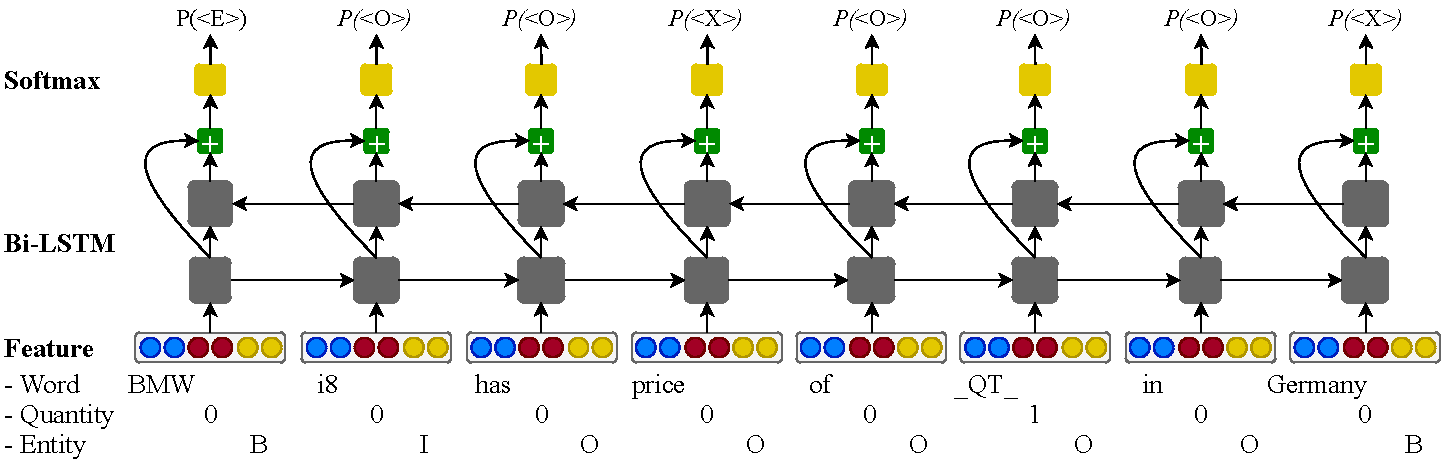
\includegraphics[width=1\textwidth]{figures/neural.pdf}
\caption{The Qfact extraction model used by Qsearch.}
\label{fig:neural}
\end{figure}
Our problem resembles the Semantic Role Labeling task \cite{DBLP:journals/coling/GildeaJ02}, which is typically addressed by
Conditional Random Fields (CRFs)
or Long Short Term Memory (LSTM) models. 
Figure \ref{fig:neural} depicts the bi-directional LSTM model 
that we devised for this task, inspired by prior work \cite{DBLP:conf/acl/HeLLZ17a}.
 Other models for sequence labeling (e.g., \cite{DBLP:conf/acl/ZhouX15, DBLP:conf/emnlp/FitzGeraldTG015})
could be easily incorporated as well. 
Our labeling network consists of three layers: Input Features, Bi-LSTM, and Softmax. 
While this general architecture is close to any other LSTM model, the most unique point here is the input representation,
as described next.

\subsubsection{Input Features.} Each token of the preprocessed input sequence is represented as the concatenation of three input feature vectors:
\begin{enumerate}[label=(\it\roman*)]
\item \textit{Word}: We include word embeddings as an input feature, which enables the neural model to 
generalize to different words having similar meanings.
In our implementation, we use Glove \cite{DBLP:conf/emnlp/PenningtonSM14} precomputed embeddings.
\item \textit{Quantity}: We provide the position of the 
pivot quantity to the model as input. 
When sentences contain multiple quantities (which is a relatively frequent case), our model operates
one quantity at a time and we re-run the model for different quantities.
%which resembles the Semantic Role Labeling task, where the verbs are passed into the input instead of the quantities.
\item \textit{Entity}: We also provide information about the recognized entities as input to the neural model. 
As entities often span multiple tokens, we employ the BIO tagging mechanism \cite{DBLP:conf/acl-vlc/RamshawM95}, where a tag \textit{B} is used for tokens at the beginning of an entity name,
\textit{I} for tokens inside the name, and \textit{O} for other tokens. 
With this representation, the output of the model only needs to tag the first token of a multi-word entity name with \textit{<E>}, 
and subsequent tokens are tagged with \textit{<O>}. Figure \ref{fig:neural} shows an example: \textit{``BMW i8''} is chosen as the entity 
connected with the pivot quantity; only the first token \textit{``BMW''} is tagged as \textit{<E>} in the output.
\end{enumerate}

\subsubsection{Output Constrained Decoding.} The output of the model are the probabilities of each token word in the input belonging to each of the three tags \textit{<E>}, \textit{<X>} and \textit{<O>}, produced by the Softmax layer. 
In neural models, usually the tag with the highest score will be assigned to each token word.
%which results in the highest probability of the whole tag sequence. 
However, this standard technique would not take into account the dependencies between output tags, and hence might give us an invalid tag sequence. To solve this issue, we impose the following two constraints on the output of the model at decoding time, and find the most probable tag sequence satisfying them: \textit{(i)} only one tag \textit{<E>} can appear in the output
(namely, for the one entity to which the pivot quantity refers);
and \textit{(ii)} that tag \textit{<E>} has to be at the start token of an entity name. 


To find the most probable tag sequence, we use Dynamic Programming to decode from left to right. Specifically, we compute subsequences of tags $\textit{Seq}_{i,j,k}$ for every $i \in \{1..n\}$ ($n$ is the sentence length)$; j \in \{\textit{<E>}, \textit{<X>}, \textit{<O>}\};$ and $k \in \{0, 1\}$. Here, $\textit{Seq}_{i,j,k}$ denotes tag subsequence with the highest probability for tokens from position $1$ to position $i$, where the tag of token at position $i$ is $j$, and the subsequence contains $k$ \textit{<E>} tags.
Note that the probability of a tag subsequence is computed as the product of the probabilities of its constituent tags. 
The final tag sequence can be derived at $i = n$.

%The final tag sequence can be derived at position $i = n$.

%We compute subsequence of tags from position 0 to i, denoted as  $\textit{Seq}_{i,j,k}$ where $i \in \{1..n\}; j \in \{\textit{<E>}, \textit{<X>}, \textit{<O>}\};$ and $k \in \{0, 1\}$. Here, $\textit{Seq}_{i,j,k}$ represents that the tag of token at position $i$ is $j$ and $k$ is interpreted as the tag subsequence with the highest probability for tokens from position $1$ to $i$.
%where the tag of token at position $i$ is $j$, and the subsequence contains $k$ \textit{<E>} tags.


\subsubsection{Distant Supervision Training.} As training data is an important factor but difficult to obtain, and manual labeling 
at scale is too 
expensive, we employ distant supervision to generate training data for the Qfact extraction model.
We use unsupervised, pattern-based Open Information Extraction (Open IE) to overlay an n-tuple structure
(with triples or higher-arity tuples) 
on the input text. 
We employ the OpenIE4 tool \cite{DBLP:conf/ijcai/Mausam16} to this end, and then use its output tuples
to generate training data. This process consists of two steps:\\

\noindent \textit{- Step 1: Capture information areas:} We define an \textit{information area} as a subset of tokens from a sentence, which presents complete information about a fact.
We run Open IE on the \textit{unprocessed} sentence to detect all possible tuples expressed by the text. 
Each of these tuples has a confidence score; to ensure the quality of the generated training samples, 
we only keep tuples having a confidence score of at least 0.9. 
Each of the selected tuples corresponds to an information area.
\begin{example} Consider the unprocessed sentence in Example \ref{ex:3}, suppose the following tuples are extracted by Open IE: (1): \textit{(BMW i8; has; price of 138k Euros; in Germany)$^{0.95}$}, (2): \textit{(BMW i8; has; range from 50 to 60 km on battery)$^{0.9}$}, (3): \textit{(BMW i8; has; price of 138k Euros)$^{0.8}$}, (4): \textit{(BMW i8; has; range from 50 to 60 km)$^{0.5}$}, and (5): \textit{(BMW i8; has; price)$^{0.1}$}. We only keep high-confidence tuples (1) and (2), which contain complete information. 
Then the following information areas are chosen for training:
{\small
\begin{align*}
\mathrlap{\underbracket{\phantom{\textit{BMW i8 has }}}_{\textit{(2)}}} \overbracket{\textit{BMW i8 has price of 138k Euros in Germany}}^{\textit{(1)}} and \underbracket{\textit{range from 50 to 60 km on battery}}_{\textit{(2)}} . \tag*{\qed}
\end{align*}
}
\end{example}
\noindent \textit{- Step 2: Transform infomation areas into training samples:} We map the information areas obtained in Step 1 with entities and quantities detected from the preprocessing phase:
{\small
\[
 \mathrlap{\underbracket{\phantom{\textit{<KB:BMW\_i8> has }}}_{\textit{(2)}}} \overbracket{\textit{<KB:BMW\_i8> has price of \_QT\_}_{(1)} \textit{in <KB:Germany>}}^{\textit{(1)}} and \underbracket{\textit{range \_QT\_}_{(2)} \textit{on battery}}_{\textit{(2)}} . \tag*{\qed}
\]
}
With this mapping, information areas yield training samples for the neural network. 
We apply conservative filters so that this self-training process minimizes spurious samples.
First, we keep only information areas that contain exactly one quantity \textit{\_QT\_}, the pivot quantity. 
Second, since English sentences tend to express quantity information in active voice, 
the entity connected to the pivot quantity should appear in the first argument (subject) of the Open IE tuple. 
For instance, information area (1) has two entities \textit{<KB:BMW\_i8>} and \textit{<KB:Germany>};
we choose the former as the one to which quantity \textit{\_QT\_$_{(1)}$} refers. 
Finally, we discard all information areas where the subject of the Open IE tuple contains more than one entity.

At this point, for each information area, we have a quantity and a unique entity to which it refers. 
The context between them is determined from the remaining tokens in the information area based on their Part-of-speech (POS) tags. 
We allow only the following POS patterns to form the context: noun (NN*), verb (VB*), adjective (JJ*), adverb (RB*), and 
foreign  word (FW, to capture out-of-vocabulary names). 
We also use pre-defined stopwords to remove uninformative tokens from the context. 
The resulting Qfact, along with the \textit{<E>,<X>,<O>} tags for its token sequence, becomes a positive training sample.
%Furthermore, to prevent the tagging model from being overly optimistic, we also take into account negative training samples, 
As negative training samples, we collect all information areas where no entity could be identified to relate with the
pivot quantity, i.e., all tokens are tagged as \textit{<O>}.


%{\tt\color{red} GW: need to say more about the actual training - size of training data, which 
%software library, batch size, epoch size, learning rate etc. !!!!!!!!!!}

 